\section{Elastic scattering calculations of a nucleon on $^{208}$Pb target} \label{part1}
\subsection{Coulomb scattering}
	In the case of point-Coulomb scattering, the Coulomb interaction between the projectile and the target with charges $Z_1$ and $Z_2$ is 
	\begin{equation}
		V_c(R)=\frac{Z_1Z_2e^2}{R^2},
	\end{equation}
	where R is the distance between them. The Schr\"{o}dinger's equation with this potential can be solved analytically. Related discussions are detailed in Ref.\cite{thompson2009nuclear}. In sum, the angular distribution of point-Coulomb potential is described by the differential cross section
	\begin{equation}\label{Ruther}
		\sigma(\theta)=\frac{\eta^2}{4k^2\sin^4(\theta/2)};\ \eta=\frac{Z_1Z_2e^2}{\hbar}\left(\frac{\mu}{2E}\right)^{\frac{1}{2}},
	\end{equation} 
	where $\mu$ is the reduced mass and $k$ is the wave number with the energy $E$. It worth noticing that the Eq. \ref{Ruther} is the same as the classical \emph{Rutherford cross section}.
	
	When the finite size of the target is included, due to different charge distributions, the interaction between the projectile and the target becomes more complicated. 
	
  	Normally, these potentials are not analytically solvable. Sometimes, we can apply the \emph{plane wave Born approximation} (PWBA) for the Coulomb scattering. Under PWBA, the differential cross section is 
  	\begin{equation}\label{ruther}
	\sigma(\theta)=\frac{\eta^2}{4k^2\sin^4(\theta/2)}\left|F(\theta)\right|^2,\end{equation}
	where $F(\theta)$ is called the \emph{form factor} related with the charge distribution as
	\begin{equation}\label{formfactor}
	F(\theta) = \int e^{i(\vec{k}_f-\vec{k}_i)\cdot\vec{r}'}\rho(r')d^3r'.
	\end{equation}
	
\subsection{Form factor of a solid sphere}
	To see substantial influence of the form factor, we give an simple example. 
	Suppose the charge distribution of the target with charge $Z_2$ is homogenous inside a solid sphere with radius $a$, which means
	\begin{align}
		\rho(R) &= \frac{3}{4\pi a^3}\ \rm{for}\ R<a\\
		&= 0\ \rm{elsewhere}.
	\end{align}
	The form factor is then calculated from Eq. \ref{formfactor}
	\begin{equation}\label{sphereformfactor}
		F(\theta)= \frac{3}{qa}\left(\frac{\sin(qa)}{(qa)^2}-\frac{\cos(qa)}{qa}\right) = \frac{3j_1(qa)}{qa}.
	\end{equation}
	where $j_1$ is spherical Bessel functions and $q=2k\sin(\theta/2)$. In Figure \ref{fig:formfactor}, we show the differential cross sections' ratio between these two cases. We can see fluctuation appears due to diffraction of finite-size body.

	 \begin{figure}[t]
		\centering
		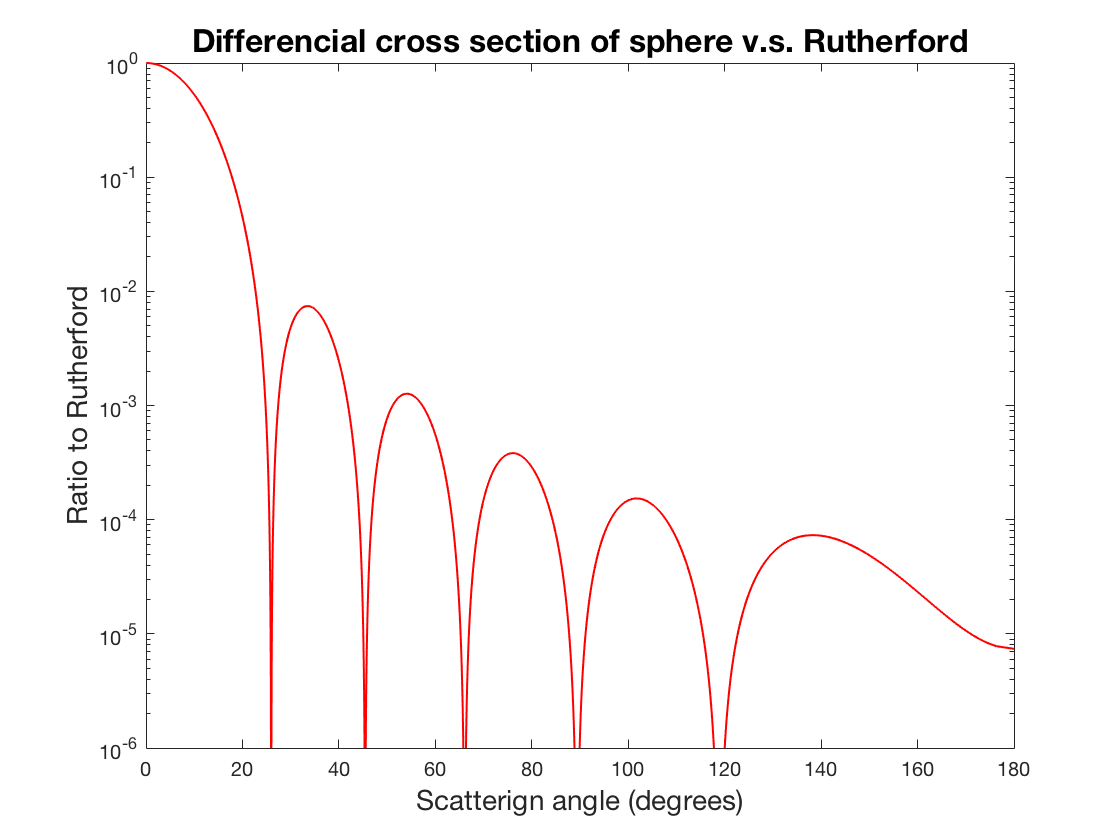
\includegraphics[width=0.5\textwidth]{1_1.png}
		\caption{Differential cross sections for solid sphere charge distribution. Here we take $a=1;k=10$.  }
		\label{fig:formfactor}
	\end{figure}
	
  	In sum, we see the finite-size target can give cross sections different from the point-like case.
\subsection{Description of elastic scattering using optical potentials}
	In this section, we study the elastic scattering between nucleons and the $^{208}$Pb target with the help of FRESCO\cite{FRESCO} . Their effective interaction is referred to as the optical potential. We take the global parameterizations from Ref. \cite{capote2009ripl,koning2003local} as the input for FRESCO.
	
	In the first step, we take two lab energies 5 and 50 (40) MeV for proton (neutron) in our calculations. The results together with experimental data are shown in Figure \ref{fig:angulardistribution}. It gives the angular distributions in center of mass for protons and neutrons. For the 5 MeV proton, the curve agrees well with the \emph{Rutherford cross section}. Given that the radius parameter of optical potential is $r_w\sim1.2\ fm$, we can estimate the Coulomb barrier for a proton to overcome. It should be 
	\begin{equation}
	E_{Coul}\approx\frac{Z_1Z_2e^2}{r_w+R_2}\approx15\ \rm{MeV}.
	\end{equation}
	We see that 5 Mev is much lower than the Coulomb barrier. Thus, this scattering can be referred as a point-like Coulomb scattering properly. The agreement with the \emph{Rutherford cross section} also verifies this point.
	For neutrons, there is no Rutherford scattering cross section to compare against, hence the value of the neutron cross section being listed as $fm^2$. At 5 MeV the cross section hints at a broad diffraction pattern.
	Since 50 MeV is strong enough to overcome the Coulomb barrier, the effective interaction plays a role and induces a diffraction pattern in Figure \ref{fig:angulardistribution}. The neutron cross section at 40 Mev exhibits a similar behavior, speaking to the dominance of the nuclear interaction at this energy. We can also see that our curves basically obey same trends as experiments. However, they deviate in values, especially for neutron. It is because we use the global parameterizations. We will include the qualitative analyses and better fittings in the next section. In order to explore the influence of the optical potential, we will use $E_{lab}$ = 50 MeV in following calculations.
	
	\begin{figure}[t]
	\centering
	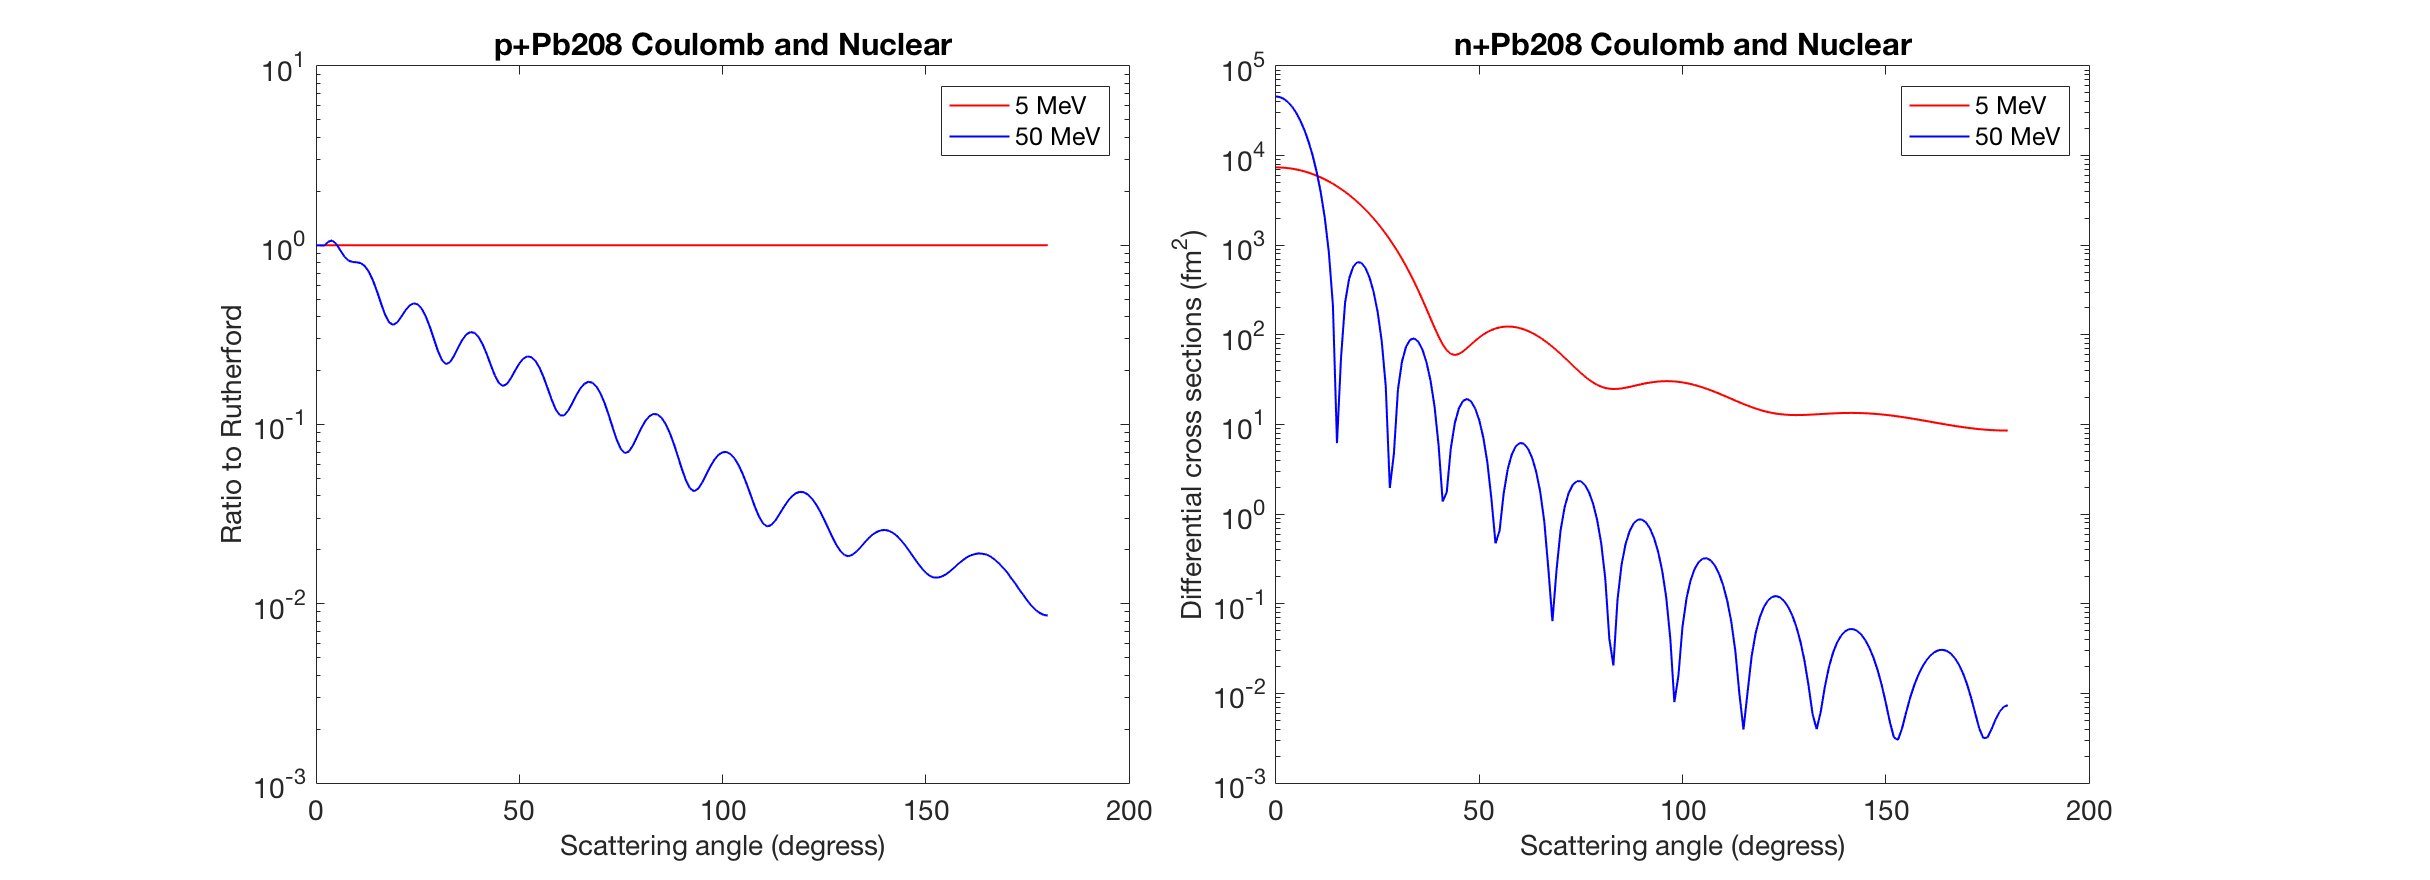
\includegraphics[width=0.92\textwidth]{5.png}
	\caption{Differential cross sections for nucleons scattering with $^{208}$Pb at 5 and 50MeV. Left panel is proton and right panel is neutron  }
	\label{fig:angulardistribution}
	\end{figure}
	
	In the next step, we would like to see the influences of the depth of optical potential's imaginary part of the S-matrix. Fixing other parameters, we scale the depth of imaginary parts $V_i$ (including volume, surface derivative and spin-orbit potentials) a factor of 1.5, 0.5 and 0. The modules of S-matrix for the proton and the neutron are shown in Table \ref{pSmatrix} and \ref{nSmatrix}. 
	We can see that as we lower the depth, $|\mathbf{S}|^2$ fluctuates and eventually converges to one which indicates an elastic scattering. It inspires us that the imaginary parts can describe absorptions in scattering processes. It also worth noticing the fluctuation of $|\mathbf{S}|^2$ with varying $V_i$ in each partial wave. For this reason, there is no simple monotonous relations between the relative depth $\bar{V}$ and the total absorptive cross section.

	\begin{table}[]
\centering
\begin{tabular}{cccccc}
\toprule
\toprule
\multicolumn{6}{c}{Proton partial waves}                                                                         \\
 \midrule
L                     & J                     & $|\mathbf{S}|^2$($\bar{V}$=1.5) & $|\mathbf{S}|^2$($\bar{V}$=1.0) & $|\mathbf{S}|^2$($\bar{V}$=0.5) & $|\mathbf{S}|^2$($\bar{V}$=0.0) \\
0                     & 0.5                   & 6.45E-04                     & 2.33E-04                     & 1.56E-02                     & 1.0                          \\
1                     & 0.5                   & 9.17E-04                     & 1.17E-03                     & 1.63E-02                     & 1.0                          \\
2                     & 1.5                   & 8.33E-04                     & 1.28E-04                     & 1.34E-02                     & 1.0                          \\
1                     & 1.5                   & 9.19E-04                     & 1.23E-03                     & 1.74E-02                     & 1.0                          \\
2                     & 2.5                   & 7.97E-04                     & 1.17E-04                     & 1.52E-02                     & 1.0                          \\
3                     & 2.5                   & 1.27E-03                     & 1.64E-03                     & 1.81E-02                     & 1.0                          \\
4                     & 3.5                   & 1.51E-03                     & 2.89E-04                     & 1.02E-02                     & 1.0                          \\
3                     & 3.5                   & 1.27E-03                     & 1.85E-03                     & 2.11E-02     
	& 1.0                          \\
   
$\cdots$           &$\cdots$                    & $\cdots$                            & $\cdots$                           & $\cdots$                           & $\cdots$                                                                \\
\bottomrule
\bottomrule
\end{tabular}
\caption{The modules of S-matrix for proton partial waves with varying imaginary potentials, where $\bar{V}$ is the scaled depth defined as $V_i(new)/V_i(initial)$.}
\label{pSmatrix}
\end{table}

\begin{table}[]
\centering
\begin{tabular}{cccccc}
\toprule
\toprule
\multicolumn{6}{c}{Neutron partial waves}                                                                         \\
 \midrule
L                     & J                     & $|\mathbf{S}|^2$($\bar{V}$=1.5) & $|\mathbf{S}|^2$($\bar{V}$=1.0) & $|\mathbf{S}|^2$($\bar{V}$=0.5) & $|\mathbf{S}|^2$($\bar{V}$=0.0) \\
0 & 0.5 & 7.88E-04                     & 1.40E-03                     & 2.16E-02                     & 1.0                            \\
1 & 0.5 & 5.24E-04                     & 4.68E-05                     & 1.75E-02                     & 1.0                            \\
2 & 1.5 & 8.94E-04                     & 1.62E-03                     & 2.29E-02                     & 1.0                            \\
1 & 1.5 & 5.24E-04                     & 4.68E-05                     & 1.75E-02                     & 1.0                            \\
2 & 2.5 & 8.94E-04                     & 1.62E-03                     & 2.29E-02                     & 1.0                            \\
3 & 2.5 & 7.27E-04                     & 1.66E-05                     & 1.67E-02                     & 1.0                            \\
4 & 3.5 & 1.15E-03                     & 1.87E-03                     & 2.51E-02                     & 1.0                            \\
3 & 3.5 & 7.27E-04                     & 1.66E-05                     & 1.67E-02                     & 1.0                            \\$\cdots$           &$\cdots$                    & $\cdots$                            & $\cdots$                           & $\cdots$                           & $\cdots$                                                                \\
\bottomrule
\bottomrule
\end{tabular}
\caption{The modules of S-matrix for neutron partial waves with varying imaginary potentials, where $\bar{V}$ is the scaled depth defined as $V_i(new)/V_i(initial)$.}
\label{nSmatrix}
\end{table}

    \begin{figure}[t]
		\centering
		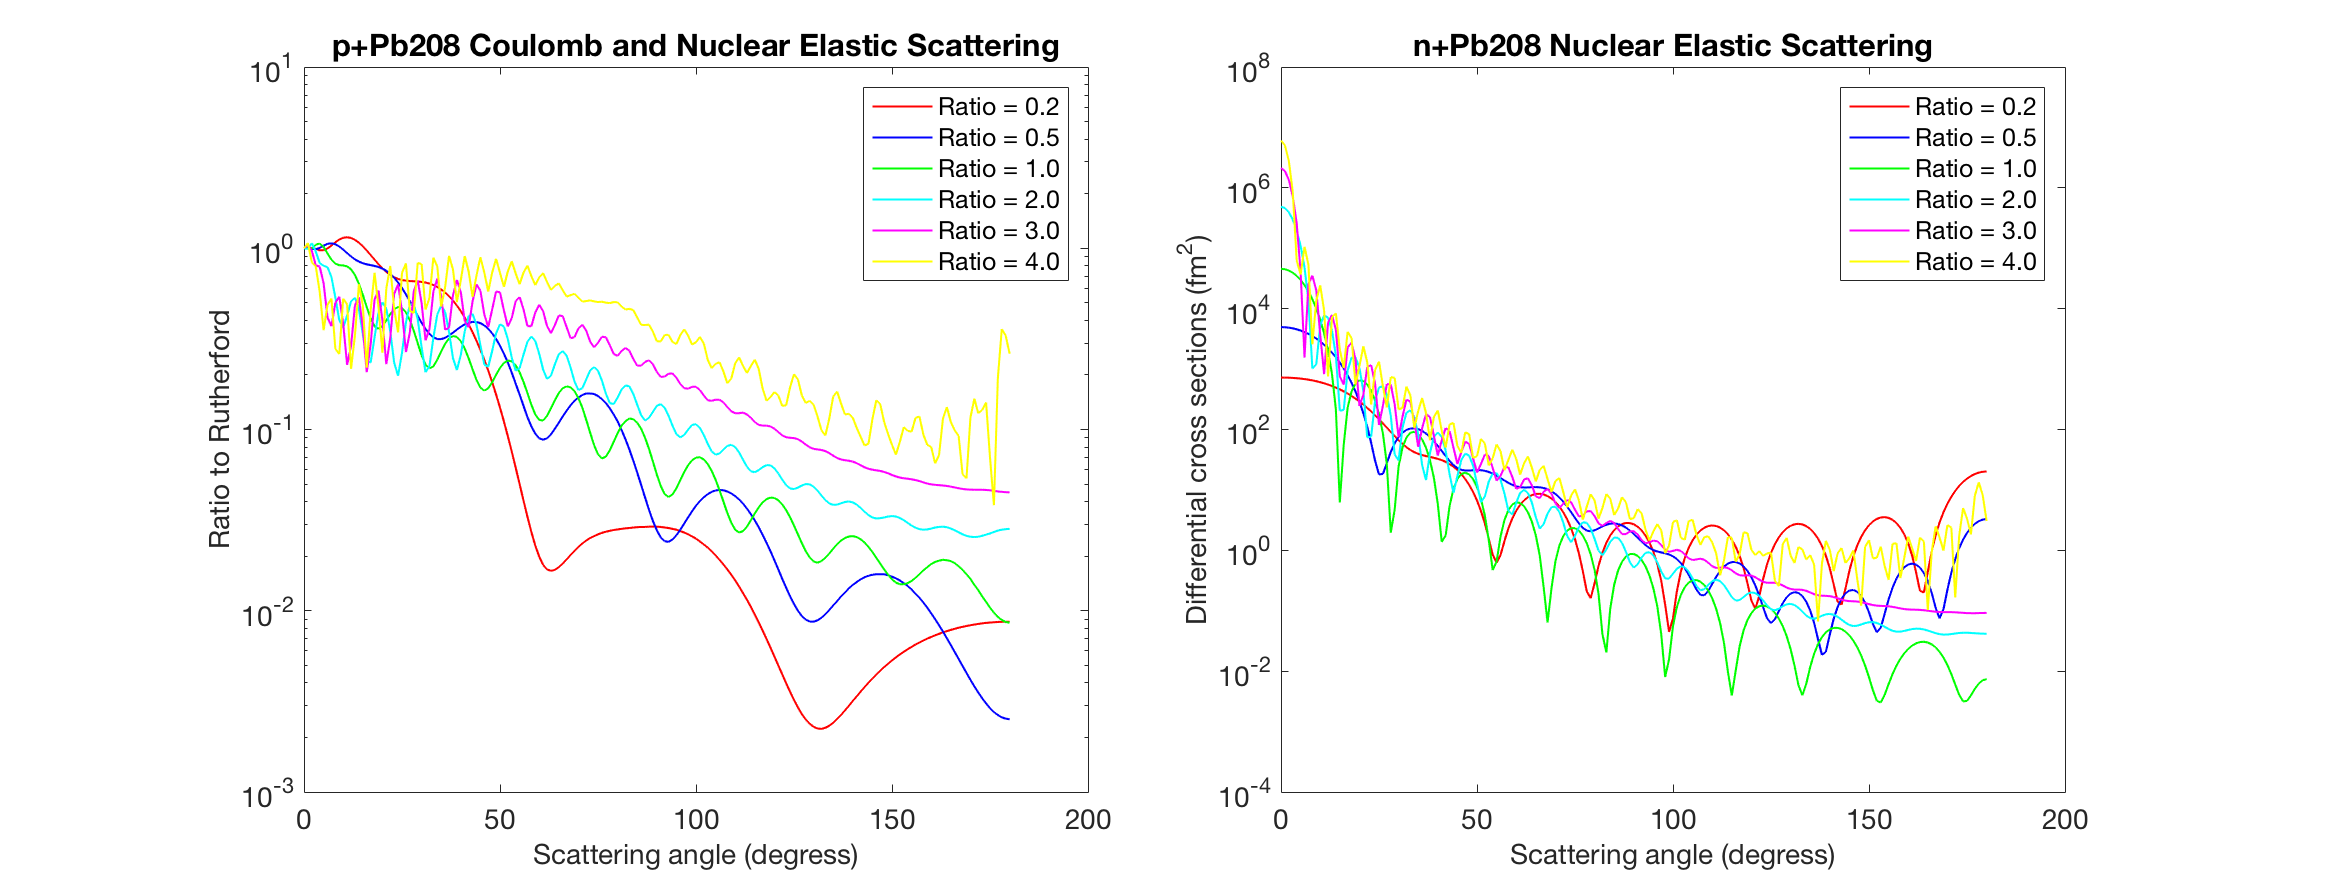
\includegraphics[width=0.92\textwidth]{7.png}
		\caption{Differential cross sections for nucleons scattering with $^{208}$Pb with different radius parameters at 50MeV, where ratio is defined as $r_{new}/r_{initial}$. Left panel is proton and right panel is neutron.  }
		\label{fig:radiusparameter}
	\end{figure}

	Moreover, we are interested in the effects brought by different radius parameters. 
	Inspired by the special situation in Eq. \ref{sphereformfactor}, since $j_1(x)$ has fixed zero points, then, as radius parameter increases, we expect a denser diffraction pattern. 
	We did't scale the Coulomb interaction at same time, so we should see stronger up-down shift for proton by it.
	
	Again, fixing other parameters, we repeat our calculations by scaling the radius parameters $r$ (including volume, surface derivative and spin-orbit potentials) a factor of 0.2, 0.5, 2, 3 and 4. 
	The results are shown in Figure \ref{fig:radiusparameter}.
	For the proton, we observe the dramatic up-down shifts and denser diffraction patterns with increasing $r$. 
	It's the synergistic effect by the Coulomb and optical potentials. 
	As for neutron, the changing of pattern is relative small as it only feels the optical potential. 
	Although the interactions are more complicated than the solid sphere, the trends in these two figures agree well with our anticipations.
	
	The total reaction cross section and the absorptive cross section are equal in a single channel elastic scattering. For neutron, we extract them according to the equation
	\begin{equation}
		\sigma_{e}=\frac{\pi}{k^2}\sum_{J}(2J+1)(1-|\mathbf{S}_J|^2).
			\end{equation}
	The total reaction and absorptive cross sections are $3.764\times 10^3$ mb. The number deviates little from the value $3.796\times 10^3$ mb given directly by FRESCO for slightly different physical constants used.
	
